%!TEX program = xelatex

%----------------------------------------------------------------------------------------
%	PACKAGES AND OTHER DOCUMENT CONFIGURATIONS
%----------------------------------------------------------------------------------------

\documentclass[
	12pt, % Default font size, select one of 10pt, 11pt or 12pt
	% fleqn, % Left align equations
	a4paper, % Paper size, use either 'a4paper' for A4 size or 'letterpaper' for US letter size
	%oneside, % Uncomment for oneside mode, this doesn't start new chapters and parts on odd pages (adding an empty page if required), this mode is more suitable if the book is to be read on a screen instead of printed
]{myLegrandOrangeBook}

% Book information for PDF metadata, remove/comment this block if not required 
\hypersetup{
	pdftitle={Title}, % Title field
	pdfauthor={Author}, % Author field
	pdfsubject={Subject}, % Subject field
	pdfkeywords={Keyword1, Keyword2, ...}, % Keywords
	pdfcreator={LaTeX}, % Content creator field
}

% 所用包
\usepackage[dvipsnames]{xcolor}
\usepackage{fancyhdr}
\usepackage{extramarks}
\usepackage{amsmath}
\usepackage{amsthm}
\usepackage{amsfonts}
\usepackage{tikz}
\usepackage[plain]{algorithm}
\usepackage{algpseudocode}
\usepackage{ctex}
\usepackage{indentfirst}
\usepackage{wrapfig}
\usepackage{upgreek}
\usepackage{subfigure}
\usetikzlibrary{automata,positioning,shapes.geometric,arrows.meta,patterns,calc}

% 我的newcommand
\newcommand{\degree}{^{\circ}}
\newcommand{\arrow}{-{Stealth[length=4mm,width=2mm]}}
\newcommand{\rmd}{\mathrm{d}}
\newcommand{\deriv}[2]{\frac{\rmd #1}{\rmd #2}}
\renewcommand{\parallel}{\mathrel{/\mskip-2.5mu/}}

\addbibresource{reference.bib} % Bibliography file

\definecolor{ocre}{RGB}{243, 102, 25} % Define the color used for highlighting throughout the book

\chapterimage{miku3.png} % Chapter heading image
\chapterspaceabove{6.5cm} % Default whitespace from the top of the page to the chapter title on chapter pages
\chapterspacebelow{6.75cm} % Default amount of vertical whitespace from the top margin to the start of the text on chapter pages

%----------------------------------------------------------------------------------------

\begin{document}

%----------------------------------------------------------------------------------------
%	TITLE PAGE
%----------------------------------------------------------------------------------------

\titlepage % Output the title page
	{\includegraphics[width=\paperwidth]{miku0.jpg}} % Code to output the background image, which should be the same dimensions as the paper to fill the page entirely; leave empty for no background image
	{ % Title(s) and author(s)
		\centering\sffamily % Font styling
		{\Huge\bfseries University Physics\par} % Book title
		\vspace{12pt} % Vertical whitespace
		{\LARGE Notes\par} % Subtitle
		\vspace{20pt} % Vertical whitespace
		{\huge\bfseries Lai Wei\par} % Author name
		\vspace{36pt} % Vertical whitespace
        {
\includegraphics[width=0.4\textwidth]{logo.png}\par}
	}

%----------------------------------------------------------------------------------------
%	献辞部分
%----------------------------------------------------------------------------------------

    \begin{dedication}
        Dedicated to {\kaishu 我自己}和{\kaishu 初音ミク}.
    \end{dedication}

%----------------------------------------------------------------------------------------
%	TABLE OF CONTENTS
%----------------------------------------------------------------------------------------

\pagestyle{empty} % Disable headers and footers for the following pages

\tableofcontents % Output the table of contents

\pagestyle{fancy} % Enable default headers and footers again

\cleardoublepage % Start the following content on a new page

%----------------------------------------------------------------------------------------
%	PART
%----------------------------------------------------------------------------------------

\part{大学物理A1}

%----------------------------------------------------------------------------------------
%	SECTIONING EXAMPLES CHAPTER
%----------------------------------------------------------------------------------------

\chapterimage{miku2.jpg} % Chapter heading image
\chapterspaceabove{6.75cm} % Whitespace from the top of the page to the chapter title on chapter pages
\chapterspacebelow{7.25cm} % Amount of vertical whitespace from the top margin to the start of the text on chapter pages

%------------------------------------------------

\chapter{质点运动学}

\section{质点力学}

\subsection{参考系、质点}

\subsubsection*{参考系}

    为描述物体运动而选的标准物。

\subsubsection*{参考系}

    物体能否视为质点视具体情况而定。

\subsubsection*{坐标系}

    定量描述物体运动。坐标系的原点一般固定在参照系上。

    \begin{enumerate}
        \item 直角坐标系\(\left(x,y,z\right)\)
        \item 球坐标系\(\left(r,\theta,\varphi\right)\):二维极坐标
        \item 柱坐标系\(\left(\rho,\varphi,z\right)\)
        \item 自然坐标系\(s\)
    \end{enumerate}

\subsection{位置矢量、运动方程、路程、位移}

\subsubsection*{位置矢量}

    \begin{wrapfigure}{r}{4cm}
        \centering
        \includegraphics[scale=0.08]{"Chapter 01 images/pic1.png"}
        % \caption{}
        \label{pic1}
    \end{wrapfigure}

    \begin{align}
        \overrightarrow{r} &= x\overrightarrow{i} + y\overrightarrow{j} + z\overrightarrow{k} \\
        r &= \left|\overrightarrow{r}\right| = \sqrt{x^2 + y^2 + z^2}
    \end{align}

    \(\overrightarrow{r}\)的方向可以用一组方向角,即\(\overrightarrow{r}\)与\(x\)轴、
    \(y\)轴、\(z\)轴之间的夹角\(\left(\alpha, \beta, \gamma\right)\)来表示。
    \(\cos \alpha = \frac{x}{r}\)、\(\cos \beta = \frac{y}{r}\)、\(\cos \gamma = \frac{z}{r}\),
    有\(\cos \alpha ^2 + \cos \beta ^2 + \cos \gamma ^2 = 1\)。

\subsubsection*{运动方程(直角坐标系下)}
    
    \begin{wrapfigure}{r}{4cm}
        \centering
        \includegraphics[scale=0.08]{"Chapter 01 images/pic2.png"}
        % \caption{}
        \label{pic2}
    \end{wrapfigure}

    \begin{align}
        \overrightarrow{r}\left(t\right) = 
        x\overrightarrow{i}\left(t\right) + y\overrightarrow{j}\left(t\right)
        + z\overrightarrow{k}\left(t\right)
    \end{align}

    分量式

    \[
    \begin{cases}
    x = x\left(t\right), \\
    y = y\left(t\right), \\ 
    z = z\left(t\right).
    \end{cases}
    \]

    从上式中消去参数得质点的{\heiti 轨迹方程}。

\subsection{位移、路程}

\subsubsection*{位移\(\Delta \overrightarrow{r}\)(位置矢量的改变量)}


    \begin{wrapfigure}{r}{4cm}
        \centering
        \includegraphics[scale=0.08]{"Chapter 01 images/pic3.png"}
        % \caption{}
        \label{pic3}
    \end{wrapfigure}

    \begin{align*}
        \overrightarrow{r_{A}} &=
        x_{A}\overrightarrow{i} + y_{A}\overrightarrow{j} + z_{A}\overrightarrow{k}
        ,\; \left(t_{A}\text{时}\right) \\
        \overrightarrow{r_{B}} &=
        x_{B}\overrightarrow{i} + y_{B}\overrightarrow{j} + z_{B}\overrightarrow{k}
        ,\; \left(t_{B}\text{时}\right)
    \end{align*}

    于是其位移

    \begin{align}
        \Delta \overrightarrow{r} = \overrightarrow{r_{B}} - \overrightarrow{r_{A}}
        = \left(x_{B} - x_{A}\right)\overrightarrow{i} + \left(y_{B} - y_{A}\right)\overrightarrow{j}
        + \left(z_{B} - z_{A}\right)\overrightarrow{k}
    \end{align}
    
    方向由\(A\)指向\(B\)。

\subsubsection*{路程\(\Delta s\)实际轨迹}

    \begin{wrapfigure}{r}{4cm}
        \centering
        \includegraphics[scale=0.05]{"Chapter 01 images/pic4.png"}
        % \caption{}
        \label{pic4}
    \end{wrapfigure}

    从\(P_{1}\)到\(P_{2}\),路程记为\(\Delta s = \hat{P_{1}P_{2}}\)。

    位移与路程的区别:

    \begin{enumerate}
        \item 位移是适量,路程是标量;
        \item 两点之间位移是唯一的,路程不是唯一的;
        \item 一般情况下,\(\left|\Delta \overrightarrow{r}\right| \neq \Delta s\)
            \\
            在方向不变的圆周运动中,\(\left|\Delta \overrightarrow{r}\right| = \Delta s\)
            当\(\Delta t \rightarrow 0\)时,\(\left| \rmd \overrightarrow{r}\right| = \rmd s\)
            (元位移\(\rmd \overrightarrow{r} = \rmd x \overrightarrow{i} +
            \rmd y \overrightarrow{j} + \rmd z \overrightarrow{k}\))。
    \end{enumerate}

\subsection{速度}

\subsubsection*{平均速度}

    \begin{wrapfigure}{r}{4cm}
        \centering
        \includegraphics[scale=0.08]{"Chapter 01 images/pic5.png"}
        % \caption{}
        \label{pic5}
    \end{wrapfigure}

    在\(\Delta t\)内,质点位移(二维)为

    \begin{align*}
        \Delta \overrightarrow{r} &= \overrightarrow{r} \left(t + \Delta t\right) -
        \overrightarrow{r} \left(t\right)
        \\
        &= \Delta x \overrightarrow{i} + \Delta y \overrightarrow{j}
    \end{align*}

    \textbf{定义}
    \begin{align}
        \overrightarrow{v} = \frac{\Delta \overrightarrow{r}}{\Delta t} =
        \frac{\Delta x}{\Delta t} \overrightarrow{i} + \frac{\Delta y}{\Delta y} \overrightarrow{j}
    \end{align}

\subsubsection*{瞬时速度}

    当\(\Delta t \rightarrow 0\)时,

    \begin{equation}
        \begin{aligned}
            \overrightarrow{v} = \lim_{\Delta t \rightarrow 0}\frac{\Delta \overrightarrow{r}}{\Delta t}
            &= \frac{\rmd \overrightarrow{r}}{\rmd t}
            \\
            &= \frac{\rmd x}{\rmd t} \overrightarrow{i} + \frac{\rmd y}{\rmd t} \overrightarrow{j}
            + \frac{\rmd z}{\rmd t} \overrightarrow{k}
            \\
            & = v_{x} \overrightarrow{i} + v_{y} \overrightarrow{j} + v_{z} \overrightarrow{k}
        \end{aligned}
    \end{equation}

    即有,

    \[
        v_{x} = \frac{\rmd x}{\rmd t},\; v_{y} = \frac{\rmd y}{\rmd t},\; v_{z} = \frac{\rmd z}{\rmd t}
    \]

    所以

    \begin{align}
        \left|\overrightarrow{v} \right| = \sqrt{\left(\frac{\rmd y}{\rmd t}\right)^2 +
        \left(\frac{\rmd y}{\rmd t}\right)^2 + \left(\frac{\rmd z}{\rmd t}\right)^2}
    \end{align}

    方向角

    \[
        \cos \alpha = \frac{v_x}{v},\; \cos \beta = \frac{v_y}{v}, \;\cos \gamma = \frac{v_z}{v}
    \]

    习惯上,二维情况下,用\(\tan \theta = \frac{v_y}{v_x}\)表示方向。

    同理,速率\(v = \frac{\rmd s}{\rmd t}\),而因为\(t \rightarrow 0\)时,
    有\(\left|\overrightarrow{r}\right| = s\),则

    \[
        v = \left|\overrightarrow{v}\right| =
        \left|\frac{\rmd \overrightarrow{r}}{\rmd t}\right|
        = \frac{\left|\rmd \overrightarrow{r}\right|}{\rmd t}
        = \frac{\rmd s}{\rmd t}
    \]

    即有,速度的大小等于速率。

\subsubsection*{速度在自然坐标系下的表示}

    \begin{align}
        \overrightarrow{v} = \frac{\rmd s}{\rmd t}\overrightarrow{e_{t}}
        = v \overrightarrow{e_{t}}
    \end{align}

    其中,\(\overrightarrow{e_{t}} = 1\),表示方向,\(v\)表示速度大小。

\subsection{加速度}

    反应速度大小和方向随时间变化快慢。

\subsubsection*{平均加速度}

    \begin{wrapfigure}{r}{4cm}
        \centering
        \includegraphics[scale=0.08]{"Chapter 01 images/pic6.png"}
        % \caption{}
        \label{pic6}
    \end{wrapfigure}


    \begin{align}
        \overline{\overrightarrow{a}} = \frac{\Delta \overrightarrow{v}}{\Delta t}
    \end{align}

    \(\overrightarrow{a}\)与\(\Delta \overrightarrow{v}\)的方向相同。

\subsubsection*{瞬时加速度}

    特点:

    \begin{enumerate}
        \item {\color{Thistle}"矢量性"}
        \item {\color{Thistle}"瞬时性"}
        \item {\color{Thistle}"相对性"}(相对于某一参考系)
    \end{enumerate}

    \begin{equation}
        \begin{aligned}
            \overrightarrow{a} &= \lim_{\Delta t \rightarrow 0} \frac{\Delta \overrightarrow{v}}{\Delta t}
            = \frac{\rmd \overrightarrow{v}}{\rmd t} =
            \frac{\rmd^2 \overrightarrow{r}}{\rmd t^2}
            \\
            &= \frac{\rmd v_{x}}{\rmd t} \overrightarrow{i} +
            \frac{\rmd v_{y}}{\rmd t} \overrightarrow{j} +
            \frac{\rmd v_{z}}{\rmd t} \overrightarrow{k}
            \\
            &= a_{x}\overrightarrow{i} + a_{y}\overrightarrow{j}
            + a_{z}\overrightarrow{k}
        \end{aligned}
    \end{equation}

    方向角\(\alpha\)、\(\beta\)和\(\gamma\)满足

    \[
        \cos \alpha = \frac{a_x}{a},\; \cos \beta = \frac{a_y}{a}, \;\cos \gamma = \frac{a_z}{a}
    \]

    习惯上,二维时方向表示为\(\tan \theta = \frac{a_y}{a_x}\)。
    
    \begin{wrapfigure}{r}{4cm}
        \centering
        \includegraphics[scale=0.05]{"Chapter 01 images/pic7.png"}
        % \caption{}
        \label{pic7}
    \end{wrapfigure}

    加速度的方向:

    \begin{itemize}
        \item 直线运动:\(\overrightarrow{a} \parallel \overrightarrow{v}\)。
        \item 曲线运动:指向轨迹凹测。
            自然坐标系下,\(\overrightarrow{a} = \overrightarrow{a_{n}} + \overrightarrow{a_{t}}\)。
    \end{itemize}

    在变速曲线运动中,加速度的方向总是指向轨迹凹的一侧。与\(\overrightarrow{v}\)呈锐角时,运动变快;
    与\(\overrightarrow{v}\)呈钝角时,运动变快。(因为\(\Delta \overrightarrow{v}\)必定指向曲线凹的一侧。)

\section{质点运动}

\subsection{一般曲线运动与圆周运动的定义}

\subsubsection*{一般曲线运动}

    特点:曲率半径随时间变化,不是定值。描述曲线运动一般选自然坐标系。

\subsubsection*{圆周运动}

    圆周运动是一种常见的、简单而基本的曲线运动,是研究一般曲线运动的基础

\subsection{圆周运动}

\subsubsection*{位置量的描述}

    \[
        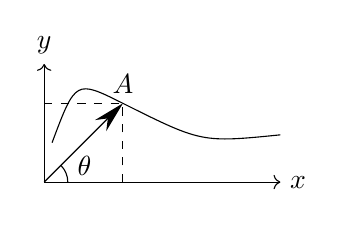
\begin{tikzpicture}
            \coordinate[label=right:$x$] (x) at (3,0);
            \coordinate[label=right:$\theta$] (theta) at (0.3,0.2);
            \coordinate[label=above:$y$] (y) at (0,1.5);
            \draw[->] (0,0) -- (x);
            \draw[->] (0,0) -- (y);
            \draw (0.1,0.5) .. controls (0.4,1.3) .. (1,1);
            \draw (1,1) .. controls (2,0.5) .. (3,0.6);
            \draw[\arrow] (0,0) -- (1,1);
            \coordinate[label=above:$A$] (A) at (1,1);
            \draw[dashed] (0,1) -- (A);
            \draw[dashed] (1,0) -- (A);
            \draw (0.3,0) arc (0:45:0.3);
        \end{tikzpicture}
    \]

    \[
        \left\{\begin{array}{l}x=r \cos \theta \\ y=r \sin \theta\end{array}\right.
    \]

    于是

    \[
        \overrightarrow{r} = x \overrightarrow{i} + y \overrightarrow{j} =
        r \cos \theta \overrightarrow{i}+ r \sin \theta \overrightarrow{j}
    \]

\subsubsection*{圆周运动的角量}

    \[
        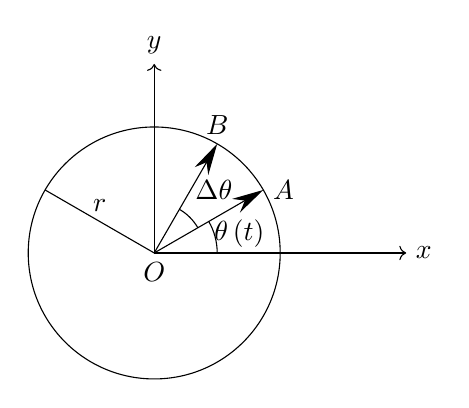
\begin{tikzpicture}[scale=0.8]
            \coordinate[label=right:$x$] (x) at (4,0);
            \coordinate[label=above:$y$] (y) at (0,3);
            \coordinate[label=below:$O$] (O) at (0,0);
            \coordinate[label=right:$A$] (A) at (1.732,1);
            \coordinate[label=above:$B$] (B) at (1,1.732);
            \coordinate[label=above:$r$] (r) at (-0.5*1.732,0.5);
            \coordinate[label={right:$\theta\left(t\right)$}] (theta) at (0.8,0.3);
            \coordinate[label=right:$\Delta \theta$] (Delta_theta) at (0.5,1);
            \draw[->] (O) -- (x);
            \draw[->] (O) -- (y);
            \draw (O) -- (-1.732,1);
            \draw[\arrow] (O) -- (A);
            \draw[\arrow] (O) -- (B);
            \draw (O) circle (2);
            \draw (1,0) arc (0:30:1);
            \draw (0.4*1.732,0.4) arc (30:60:0.8);
        \end{tikzpicture}
    \]

    角坐标\(\theta\left(t\right)\),角位移\(\Delta \theta = \theta\left(t\right) -
    \theta\left(t_0\right)\)。

    平均角速度
    
    \begin{align}
        \overline{\omega} = \frac{\Delta \theta}{\Delta t}
    \end{align}
    
    角速度
    
    \begin{align}
        \omega = \lim_{\Delta t \rightarrow 0} \frac{\Delta \theta}{\Delta t}
        = \deriv{\theta}{t}
    \end{align}

    \(\omega\)是\textbf{赝矢量},方向与\(\rmd \theta\)一致,由右手螺旋定则确定,
    且总是垂直于圆平面,沿着圆周的轴线方向。

    平均角加速度
    
    \begin{align}
        \overline{\alpha} = \frac{\Delta \omega}{\Delta t}
    \end{align}
    
    角加速度
    
    \begin{align}
        \alpha = \lim_{\Delta t \rightarrow 0} \frac{\Delta \omega}{\Delta t}
        = \deriv{\omega}{t} = \frac{\rmd^2 \theta}{\rmd t^2}
    \end{align}

\subsubsection*{角量与线量的关系}

    路程与角距离的关系

    \begin{align}
        \Delta s = r \Delta \theta
    \end{align}

    速率与角速度的关系

    \begin{align*}
        b = \lim_{\Delta t \rightarrow 0} \frac{\Delta s}{\Delta t}
        = r \lim_{\Delta t \rightarrow 0} \frac{\Delta \theta}{\Delta t}
    \end{align*}

    故

    \begin{align}
        v \left(t\right) = r \omega \left(t\right)
    \end{align}

    速度

    \begin{equation}
        \begin{aligned}
            \overrightarrow{v} &= \deriv{s}{t} \overrightarrow{e_t} \\
            &= v \overrightarrow{e_t} \\
            &= r \omega \overrightarrow{e_t}
        \end{aligned}
    \end{equation}

\subsubsection*{圆周运动的切向加速度和法向加速度}

    \[
        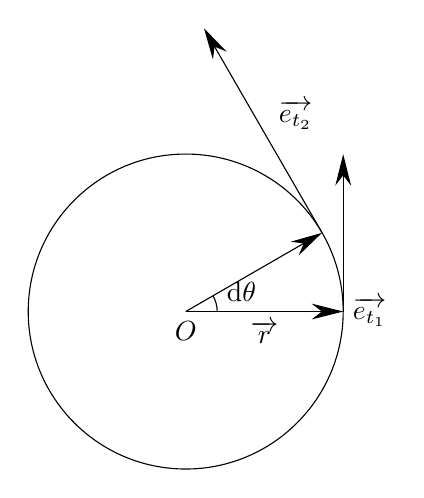
\begin{tikzpicture}
            \coordinate[label=below:$O$] (O) at (0,0);
            \coordinate[label=right:$\rmd \theta$] (dtheta) at (0.4,0.25);
            \coordinate[label=below:$\overrightarrow{r}$] (r) at (1,0);
            \coordinate[label=right:$\overrightarrow{e_{t_1}}$] (e_t_1) at (2,0);
            \coordinate[label=left:$\overrightarrow{e_{t_2}}$] (e_t_2) at (1.732,2.5);
            \draw (O) circle (2);
            \draw[\arrow] (O) -- (e_t_1);
            \draw[\arrow] (O) -- (1.732,1);
            \draw[\arrow] (e_t_1) -- (2,2);
            \draw[\arrow] (1.732,1) -- (1.732-1.5,1+1.5*1.732);
            \draw (0.4,0) arc (0:30:0.4);
        \end{tikzpicture}
    \]

    质点做变速圆周运动时

    \begin{equation}
        \overrightarrow{\alpha}=\deriv{\overrightarrow{v}}{t}=
        \frac{\rmd}{\rmd t}\left(v \overrightarrow{e}_t\right)=\deriv{\overrightarrow{v}}{t}
        \overrightarrow{e}_t+\overrightarrow{v} \deriv{\overrightarrow{e}_t}{t}
    \end{equation}

    \begin{equation}
        \alpha_{t} = \deriv{v}{t} = r \deriv{\omega}{t} = r \alpha
    \end{equation}

    因为\(\left|e_{t_1}\right| = \left|e_{t_2}\right| =1\),所以\(\left|\rmd \overrightarrow{e}\right|
    = \left|\overrightarrow{e_{t_1}}\right| \cdot \rmd \theta = \rmd \theta\)。

    当\(\rmd \theta \rightarrow 0\)时,\(\rmd \overrightarrow{e_{t}} \perp \overrightarrow{e_{t_1}}\),
    故\(\rmd \overrightarrow{e_{t}}\)的方向与\(\overrightarrow{e_{n}}\)方向相同,即

    \begin{align}
        \rmd \overrightarrow{e_{t}} = \rmd \theta \overrightarrow{e_n}
    \end{align}

    所以

    \[
        v \deriv{\overrightarrow{e_t}}{t} = v \deriv{\theta}{t} \overrightarrow{e_{n}} = v \omega
    \]

    于是

    \begin{align}
        \alpha_n &= \omega v \\
        &= \frac{v^2}{r}
    \end{align}

    综上所述,切向加速度\(\overrightarrow{\alpha_t} = \deriv{v}{t} \overrightarrow{e_t}, \;
    \alpha_t = \deriv{v}{t}\);法向加速度\(\overrightarrow{\alpha_t} = \frac{v^2}{r} \overrightarrow{e_n},
    \; \alpha_n = \frac{v^2}{r} = \omega^2r = \omega v\)。

\subsection{一般曲线运动}

    同圆周运动理知,

    \begin{align}
        \alpha_t = \deriv{v}{t}
    \end{align}

    \begin{align}
        \alpha_n = \frac{v^2}{\rho}\; \text{(\(\rho\)是曲率半径)}
    \end{align}

    而\(\overrightarrow{\alpha} = \overrightarrow{\alpha_t} + \overrightarrow{\alpha_n}\),所以

    \begin{align}
        \left|\overrightarrow{\alpha}\right| = \sqrt{\alpha_t^2 + \alpha_n^2}
    \end{align}

    自然坐标系下的加速度表达式:
    
    \begin{align}
        \overrightarrow{\alpha_t} = \deriv{v}{t} \overrightarrow{e_t} =
        \frac{\rmd^2 s}{\rmd t^2} \overrightarrow{e_t}
    \end{align}

    \begin{align}
        \overrightarrow{\alpha_n} = \frac{v^2}{\rho} \overrightarrow{e_n}
    \end{align}

\section{相对运动}

\subsection{时间与空间}

    在两个相对作直线运动的参考系中,时间的测量是绝对的,空间的测量也是绝对的,与参考系无关。

    时间和长度的的绝对性是经典力学或牛顿力学的基础。

    在两个相对作直线运动的参考系中, 时间的测量是绝对的,空间的测量也是绝对的, 与参考系无关, 时间和长度的的绝对性是经典力学或牛顿力学的基础。

\subsection{相对运动公式}

    \begin{wrapfigure}{r}{4cm}
        \centering
        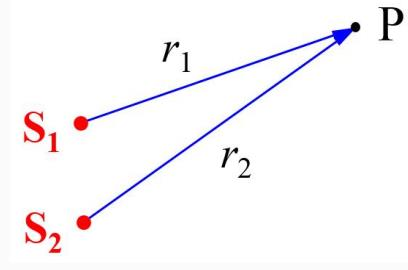
\includegraphics[scale=0.3]{"Chapter 01 images/pic8.png"}
        % \caption{}
        \label{pic8}
    \end{wrapfigure}

    如右图,\(\overrightarrow{r_{OP}} = \overrightarrow{r_{OO^{'}}} + \overrightarrow{r_{O^{'}P}}\),

    对方程两边对时间求导数,得

    \begin{align*}
        \deriv{\overrightarrow{r_{OP}}}{t} = \deriv{\overrightarrow{r_{OO^{'}}}}{t} +
        \deriv{\overrightarrow{r_{O^{'}P}}}{t}
    \end{align*}

    即

    \begin{align}
        \overrightarrow{v_{P \rightarrow O}} = \overrightarrow{v_{P \rightarrow O^{'}}} +
        \overrightarrow{v_{O^{'} \rightarrow O}}
    \end{align}

    (绝对速度 = 相对速度 + 牵连速度)

    方程两边对时间求导数,得

    \begin{align}
        \overrightarrow{a_{P \rightarrow O}} = \overrightarrow{a_{P \rightarrow O^{'}}} +
        \overrightarrow{a_{O^{'} \rightarrow O}}
    \end{align}

    (绝对加速度 = 相对加速度 + 牵连加速度)

    如果\(\overrightarrow{u}\)是恒矢量,则\(\deriv{\overrightarrow{u}}{t} = 0\),
    \(\overrightarrow{a_{PO}} = \overrightarrow{a_{PO^{'}}}\),\(\overrightarrow{a_{O^{'}O}} = 0\)。

    注意:

    \begin{enumerate}
        \item 当\(\overrightarrow{u}\)接近光速时,速度变换、加速度变换不成立;
        \item 仅仅讨论\(\overrightarrow{u} = u_x \overrightarrow{i}\)的情况(\(u_x\)为常数),
        即水平方向有变换,其他方向上没有变换。
    \end{enumerate}

\subsection{伽利略速度变换}

    \begin{wrapfigure}{r}{4cm}
        \centering
        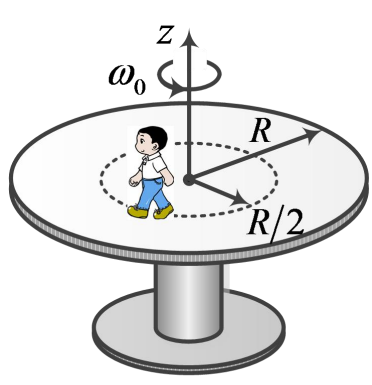
\includegraphics[scale=0.4]{"Chapter 01 images/pic9.png"}
        % \caption{}
        \label{pic9}
    \end{wrapfigure}

    \begin{align}
        \overrightarrow{v} = \overrightarrow{v}^{'} + \overrightarrow{u}
    \end{align}

    绝对速度\(\overrightarrow{v} = \deriv{\overrightarrow{r}}{t}\),相对速度\(\overrightarrow{v}^{'} =
    \deriv{\overrightarrow{r}^{'}}{t}\),牵连速度\(\overrightarrow{u}\)。

    加速度关系:

    \begin{align}
        \deriv{\overrightarrow{v}}{t} = \deriv{\overrightarrow{v}^{'}}{t} + \deriv{\overrightarrow{u}}{t}
    \end{align}

    若\(\deriv{\overrightarrow{u}}{t} = 0\),则\(\overrightarrow{a} = \overrightarrow{a}^{'}\)

\section{例题}

\subsection{Problem 1}

    在离水面高为\(h\)的岸上,有人用绳拉船靠岸,如图所示。设人以匀速率\(v_{0}\)收绳,试求:
    当船距岸边\(x_{0}\)时,船的速度和加速度的大小各是多少?

    \[
        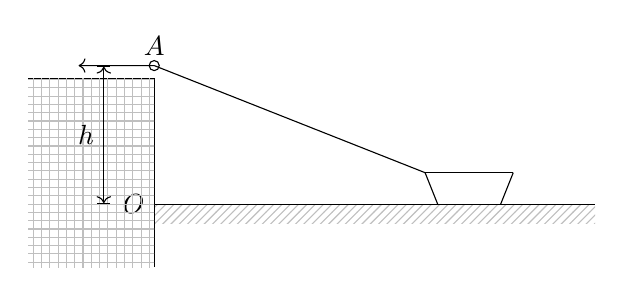
\begin{tikzpicture}[scale=0.8]
            \coordinate[label=left:$O$] (O) at (0,0);
            \coordinate[label=above:$A$] (A) at (0,2.2);
            \fill[pattern=north east lines, pattern color=gray!50] (0,0) rectangle (7,-0.3);
            \draw (0,-1) -- (0,2);
            \draw (O) -- (7,0);
            \draw (0,2) -- (-2,2);
            \fill[pattern=grid, pattern color=gray!50] (0,-1) rectangle (-2,2);
            \draw (A) circle (0.08);
            % 小船
            \draw (4.5,0) -- (5.5,0);
            \draw (4.5,0) -- (4.3,0.5);
            \draw (5.5,0) -- (5.7,0.5);
            \draw (4.3,0.5) -- (5.7,0.5);
            % 绳子
            \draw (A) -- (4.3,0.5);
            \draw[->] (A) -- (-1.2,2.2);
            % 尺寸标注
            \draw[|<->|] (-0.8,0) -- (-0.8,2.2) node[midway, left] {$h$};
        \end{tikzpicture}
    \]
    \\

    \textbf{Solution}
    \\

    \textbf{Part One}

    建立如图所示的坐标系。

    \[
        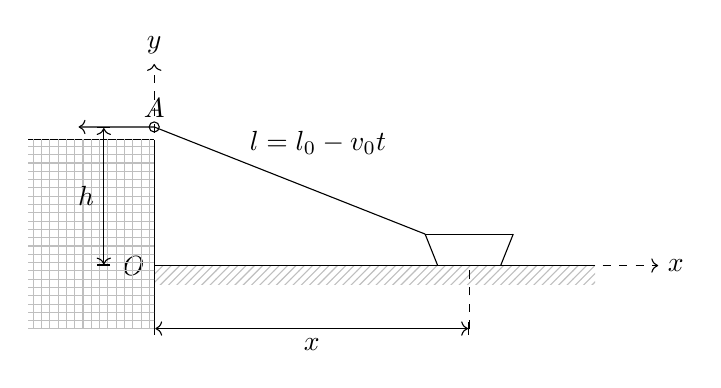
\begin{tikzpicture}[scale=0.8]
            \coordinate[label=left:$O$] (O) at (0,0);
            \coordinate[label=above:$A$] (A) at (0,2.2);
            \fill[pattern=north east lines, pattern color=gray!50] (0,0) rectangle (7,-0.3);
            \draw (0,-1) -- (0,2);
            \draw (O) -- (7,0);
            \draw (0,2) -- (-2,2);
            \fill[pattern=grid, pattern color=gray!50] (0,-1) rectangle (-2,2);
            \draw (A) circle (0.08);
            % 小船
            \draw (4.5,0) -- (5.5,0);
            \draw (4.5,0) -- (4.3,0.5);
            \draw (5.5,0) -- (5.7,0.5);
            \draw (4.3,0.5) -- (5.7,0.5);
            % 绳子
            \draw (A) -- (4.3,0.5);
            \draw[->] (A) -- (-1.2,2.2);
            \coordinate[label={above:$ l = l_{0} - v_{0}t $}] (rope) at (2.6,1.6);
            % 尺寸标注
            \draw[|<->|] (-0.8,0) -- (-0.8,2.2) node[midway, left] {$h$};
            \draw[|<->|] (0,-1) -- (5,-1) node[midway, below] {$x$};
            \draw[dashed] (5,-1) -- (5,0);
            % 坐标系
            \coordinate[label=right:$x$] (x) at (8,0);
            \coordinate[label=above:$y$] (y) at (0,3.2);
            \draw[->,dashed] (O) -- (x);
            \draw[->,dashed] (O) -- (y);
        \end{tikzpicture}
    \]

    设初始时刻,船与岸上\(A\)点之间的绳长为\(l_{0}\)。在任意时刻船离岸边的距离为\(x\),
    绳长为\(l_{0}\)。船在运动过程中,\(l\)和\(x\)均是时间\(t\)的函数。

    由题意,\(l = l_{0} - v_{0}t\),所以

    \[
        v_{0} = - \deriv{l}{t}
    \]

    又由几何关系

    \[
        l^{2} = x^{2} + h^{2}
    \]

    对上式两边同时对\(t\)求导,可得

    \[
        2 l \deriv{l}{t} = 2x \deriv{x}{t}
    \]

    则船的运动速度为

    \[
        v = \deriv{x}{t} = \frac{l}{x} \deriv{l}{t} = -\frac{l}{x} v_{0}
    \]
    \\

    \textbf{Part Two}

    再将速度对时间\(t\)求导,即可得到船的加速度为

    \[
        a = \deriv{v}{t} = - \frac{v_{0}}{x^{2}} \left(x \deriv{l}{t} - l \deriv{x}{t}\right)
        = -\frac{v_{0}^{2} h^{2}}{x^{3}}
    \]
    \\

    \textbf{Part Three}

    令\(x=x_{0}\),得船在离岸边为\(x_{0}\)时的速度和加速度分别为

    \[
        v = \frac{\sqrt{x_{0}^{2} + h^2}}{x_{0}} v_{0},\;
        a = -\frac{v_{0}^{2} h^{2}}{x_{0}^{3}}
    \]

\chapter{牛顿运动定律}

\section{牛顿定律}

\subsection{牛顿第一定律}

    牛顿第一定律,又称惯性定律(law of inertia) 可表述如下:任何物体都将保持静止
    或匀速直线运动的状态,直至其他物体的作用强迫它改变这种状态时为止。

    即当\(\overrightarrow{F} = 0\)时,\(\overrightarrow{v}\)为恒矢量。

    牛顿第一定律指出了两个重要概念\textbf{惯性}和\textbf{力}。

\subsection{牛顿第二定律}

\subsubsection{表述}

    动量为\(\overrightarrow{p}\)的物体, 在合外力\(\overrightarrow{F} \left(=\sum \overrightarrow{F_{i}}\right)\)
    的作用下,其动量随时间的变化率应当等于作用于物体的合外力,即

    \begin{align}
        \overrightarrow{F}\left(t\right) = \deriv{\overrightarrow{p}\left(t\right)}{t} =
        \deriv{\left(m\overrightarrow{v}\right)}{t}
    \end{align}

    (当\(v\ll c\)时,\(m\)为常量)

    于是有

    \begin{align}
        \overrightarrow{F} = m \deriv{\overrightarrow{v}}{t} = m \overrightarrow{a}
    \end{align}

    即可叙述如下:物体受到外力作用时,它所获得的加速度的大小与外力的大小成正比,
    与物体的质量成反比,加速度的方向与外力的方向相同。

\subsubsection{牛顿运动定律的矢量性}

    由

    \begin{align*}
        \overrightarrow{F} = m \deriv{\overrightarrow{v}}{t} = m \overrightarrow{a}
    \end{align*}

    得

    \begin{equation}
        \overrightarrow{F}=m \frac{\mathrm{~d} v_x}{\mathrm{~d} t} \overrightarrow{i}+m \frac{\mathrm{~d} v_y}{\mathrm{~d} t} \overrightarrow{j}+m \frac{\mathrm{~d} v_z}{\mathrm{~d} t} \overrightarrow{k}
    \end{equation}

    即

    \begin{equation}
        \overrightarrow{F}=m a_x \overrightarrow{i}+m a_y \overrightarrow{j}+m a_z \overrightarrow{k}
    \end{equation}

    所以

    \begin{equation}
        \left\{\begin{array}{l}
        F_x=m a_x \\
        F_y=m a_y \\
        F_z=m a_z
        \end{array}\right.
    \end{equation}

\subsubsection{自然坐标系中}

    \begin{equation}
        \overrightarrow{F}=m \overrightarrow{a}=
        m\left(\overrightarrow{a}_{\mathrm{t}}+\overrightarrow{a}_{\mathrm{n}}\right)=
        m \frac{\mathrm{~d} v}{\mathrm{~d} t} \overrightarrow{e}_{\mathrm{t}}+m \frac{v^2}{\rho} \overrightarrow{e}_{\mathrm{n}}
    \end{equation}

    也可写作

    \begin{equation}
        \left\{\begin{array}{l}
        F_{\mathrm{t}}=m \frac{\mathrm{~d} v}{\mathrm{~d} t}=m \frac{\mathrm{~d} s^2}{\mathrm{~d} t^2} \\
        F_{\mathrm{n}}=m \frac{v^2}{\rho}
        \end{array}\right.
    \end{equation}

    (\(\rho\)为\(A\)处曲线的曲率半径)

\subsubsection{力的叠加原理}

    当一个物体同时受到几个力的作用时,则这些力的合力产生的加逃度等于每个力单独作用时产生的矢
    量和,这一结论称为力的\textbf{独立性原理}或\textbf{力的叠加原理}。

    即

    \begin{equation}
        \begin{aligned}
        \overrightarrow{F} & =\overrightarrow{F}_1+\overrightarrow{F}_2+\cdots+\overrightarrow{F}_n=\sum \overrightarrow{F}_i \\
        & =m \overrightarrow{a}_1+m \overrightarrow{a}_2+\cdots+m \overrightarrow{a}_n=m \sum \overrightarrow{a}_i=m \overrightarrow{a}=m \frac{\mathrm{~d} v}{\mathrm{~d} t}
        \end{aligned}
    \end{equation}

\subsection{牛顿第三定律}

    两个物体之间作用力\(\overrightarrow{F}\)反和反作用力\(\overrightarrow{F}^{'}\), 
    沿同一直线,大小相等,方向相反,分别作用在两个物体上。

    作用力和反作用力的特点:

    \begin{enumerate}
        \item 作用力与反作用力总是同时存在、相互依存的。
        \item 作用力与反作用力分别作用在两个不同的物体上,虽然它们大小相等、方向相反,但不能互相抵消。
        \item 作用力与反作用力一定属于同一性质的力。
    \end{enumerate}

\subsection{总结}

    \begin{enumerate}
        \item 凡相对于惯性系作匀速直线运动的一切参考系都是惯性系;
        \item 对于不同惯性系,牛顿力学的规律都具有相同的形式,与惯性系的运动无关。
            (\textbf{伽利略相对性原理}或称\textbf{力学相对性原理})
    \end{enumerate}

\section{非惯性系、惯性力}

\subsection{惯性系、非惯性系}

\subsubsection{惯性系}

    牛顿运动定律在其中成立的参考系称为\textbf{惯性参考系},简称\textbf{惯性系}(inertial system)。

    “一个远离其他一切物体,而且没有自转的物体是惯性参照系,一切相对于该物体做匀速直线运动的参照系也是惯性参照系。
    牛顿定律就是在这样的参照系中成立。”——王燕生教授《大学物理问题讨论集》

    \textbf{举例}:

    \begin{enumerate}
        \item 地面参考系;
        \item 地心参考系;
        \item 日心参考系;
        \item FK4参考系:以选定的1535颗恒星的平均静止的位形作为基准的参考系,是比以上三个参考系都严格的惯性系。
    \end{enumerate}

\subsubsection{非惯性系}

    牛顿运动定律不成立的参考系称为\textbf{非惯性系}(non-inertial system)。

\subsection{惯性力}

\subsection{平动加速参考系、平动惯性力}

\subsubsection{定义}

    假设非惯性系K'相对于惯性系K以加速度\(\overrightarrow{a}_{0}\)做平动,则由相对运动规律可知,质点相对于
    K'系和K系的加速度\(\overrightarrow{a}_{0}\)和\(\overrightarrow{a}\)满足:

    \begin{align}
        \overrightarrow{a} = \overrightarrow{a}_{0} + \overrightarrow{a}^{'}
    \end{align}

    惯性系中K,牛顿运动定律成立,即

    \begin{align}
        \overrightarrow{F} = m \overrightarrow{a} = m \left(\overrightarrow{a}_{0} + \overrightarrow{a}^{'}\right)
    \end{align}

    移项,得

    \begin{align}
        \overrightarrow{F} - m\overrightarrow{a}^{'} =  m \overrightarrow{a}_{0}
    \end{align}

    定义\textbf{平动惯性力}:

    \begin{align}
        \overrightarrow{F}_{0} = - m\overrightarrow{a}^{0}
    \end{align}

    将\(\overrightarrow{F}^{'} = \overrightarrow{F} + \overrightarrow{F}_{0} = \overrightarrow{F} -
    m \overrightarrow{a}_{0}\)看作非惯性参考系中受到的“合外力”,则在非惯性系K'中,牛顿第二定律在形式上成立:

    \begin{align}
        \overrightarrow{F}^{'} = \overrightarrow{F} + \overrightarrow{F}_{0} = m \overrightarrow{a}^{'}
    \end{align}

\subsubsection{性质}

    不是真实的力,无施力物体,无反作用力是非惯性系加速度的反映。

\subsection{匀速转动参考系、惯性离心力}
    
    \begin{wrapfigure}{r}{4cm}
        \centering
        \includegraphics[scale=0.2]{"Chapter 02 images/pic1.jpg"}
        % \caption{}
        \label{pic1}
    \end{wrapfigure}

    匀速转动参考系也是一种常见的非惯性系。如右图所示,水平转盘以匀角速度\(\omega\)绕通过圆心的垂直轴转动,
    质量为\(m\)的小球用长度为\(R\)的绳子与转轴相连静止在圆盘上,并随圆盘一起转动。站在地面上的观察者看来,
    小球\(m\)以匀角速度\(\omega\)随圆盘一起转动,绳子施于小球的拉力\(\overrightarrow{F}_{r}\)
    提供了小球做匀速圆周运动时所需的向心力,即

    \begin{align}
        \overrightarrow{F}_{\mathrm{T}}=-m \frac{v^2}{R} \overrightarrow{e}_r=-m \omega^2 R \overrightarrow{e}_r
    \end{align}

    这表明在地面参考系中,小球的运动符合牛顿运动定律。

    但是,从圆盘这个转动参考系中来看,小球受到合外力\(\overrightarrow{F}_{T}\)的作用,但是静止不动。
    为了在转动参考系中,仍然能够用牛顿运动定律解释该现象,需要引入一个虛拟的惯性力\(\overrightarrow{F}_{0}\),
    该力与绳子的拉力\(\overrightarrow{F}_{T}\)大小相等、方向相反,即

    \begin{equation}
        \overrightarrow{F}_0=-\overrightarrow{F}_{\mathrm{T}}=m \omega^2 R \overrightarrow{e}_r=-m \overrightarrow{a}_{\mathrm{n}}
    \end{equation}

    (\(\overrightarrow{e}_r\)表示径向单位矢量)

    称为\textbf{惯性离心力}(inertial centrifugal force)。

    于是引入惯性离心力后,在转动参考系中,牛顿运动定律在形式上成立。物体受到“合外力”为

    \begin{align*}
        \overrightarrow{F}_{T} + \overrightarrow{F}_{0} = \overrightarrow{0}
    \end{align*}

\section{例题}

\subsection{解题思路}

    牛顿定律主要处理两类问题:

    \begin{enumerate}
        \item 质点;
        \item 质点系,尤其是连续分布的质点系。
    \end{enumerate}

    解题的基本思路:

    \begin{enumerate}
        \item 确定研究对象进行受力分析(隔离物体,画受力图);
        \item 取坐标系;
        \item 列方程(一般用分量式);
        \item 利用其它的约束条件列补充方程;
        \item 先用文字符号求解,后带入数据计算结果。
    \end{enumerate}

\subsection{Problem 1}

    一质量\(m\),半径\(r\)的球体在水中静止释放沉入水底。已知阻力\(F_{r} = - 6 \uppi r \eta v\),
    \(\eta\)为粘滞系数,求\(v\left(t\right)\)。
    \vspace{1em}

    \textbf{Solution}
    \vspace{1em}

    \begin{wrapfigure}{r}{4cm}
        \centering
        \includegraphics[scale=0.3]{"Chapter 02 images/pic2.png"}
        % \caption{}
        \label{pic2}
    \end{wrapfigure}

    取坐标如图(\(\overrightarrow{F}_{B}\)为浮力),则

    $$
        m g-F_{\mathrm{B}}-6 \uppi \eta r v=m a
    $$

    令\(F_{0} = mg - F_{B}\),\(b = 6 \uppi \eta r\),于是

    $$
        F_0-b v=m \frac{\mathrm{~d} v}{\mathrm{~d} t}
    $$

    即

    $$
        \frac{\mathrm{d} v}{\mathrm{~d} t}=-\frac{b}{m}\left(v-\frac{F_0}{b}\right)
    $$

    两边同时积分:

    $$
        \int_0^v \frac{\rmd v}{v-\left(\frac{F_0}{b}\right)}=-\frac{b}{m} \int_0^t \rmd t
    $$

    得

    $$
        v=\frac{F_0}{b}\left[1-\mathrm{e}^{-\frac{b}{m} t}\right]
    $$

    \begin{wrapfigure}{r}{4cm}
        \centering
        \includegraphics[scale=0.3]{"Chapter 02 images/pic3.png"}
        % \caption{}
        \label{pic3}
    \end{wrapfigure}

    则当\(t \rightarrow \infty\)时,\(v_{L} \rightarrow \frac{F_{0}}{b}\)(极限速度),
    当\(t = 3 \frac{b}{m}\)时,\(v = v_{L}\left(1-0.05\right) = 0.95 v_{L}\)。
    一般认为\(t \leq 3 \frac{b}{m}\)时,\(v = v_{L}\)

\subsection{Problem 2}

    质量为\(m\)的物体,由地面以初速度\(v_{0}\)竖直向上发射,物体受到空气阻力大小\(F_{r} = kv\)。
    试求:

    \begin{enumerate}
        \item 物体发射到最大高度所需要的时间;
        \item 物体能到达的最大高度。
    \end{enumerate}

    \textbf{Solution}
    \\

    \textbf{Part One}
    \\

    \begin{wrapfigure}{r}{4cm}
        \centering
        \includegraphics[scale=0.3]{"Chapter 02 images/pic4.png"}
        % \caption{}
        \label{pic4}
    \end{wrapfigure}

    物体在向上发射的过程中,受到重力和阻力作用,方向均与速度方向相反。以竖直向上作为正方向,
    由牛顿运动定律可得

    \begin{equation}
        -m g-k v=m \frac{\mathrm{~d} v}{\mathrm{~d} t}
        \label{Problem-2-1}
    \end{equation}

    对上式分离变量并取定积分,同时注意到物体到达最大高度时\(v=0\),即

    $$
        \int_0^t \mathrm{~d} t=\int_{v_0}^0-\frac{m}{m g+k v} \mathrm{~d} v
    $$

    积分得物体达到最大高度所需的时间为

    $$
        t=\frac{m}{k} \ln \frac{m g+k v_0}{m g}
    $$

    \textbf{Part Two}
    \\

    利用$\dfrac{\mathrm{d} v}{\mathrm{~d} t}=v \dfrac{\mathrm{~d} v}{\mathrm{~d} y}$代入\ref{Problem-2-1}式,可得

    $$
        -m g-k v=m \frac{\mathrm{~d} v}{\mathrm{~d} t}
    $$

    分离变量并取定积分,即

    $$
        \int_0^y \mathrm{~d} y=\int_{v_0}^0-\frac{m v}{m g+k v} \mathrm{~d} v
    $$

    所以物体可达到的最大高度为

    $$
        y=\frac{m}{k}\left(v_0-\frac{m g}{k} \ln \frac{m g+k v_0}{m g}\right)
    $$

\subsection{Problem 3}

    \begin{wrapfigure}{r}{4cm}
        \centering
        \includegraphics[scale=0.18]{"Chapter 02 images/pic5.png"}
        % \caption{}
        \label{pic5}
    \end{wrapfigure}

    一条质量均匀分布的绳子,总质量为\(M\)、长度为\(L\),一端拴在竖直转轴\(OO^{'}\)上,
    并以恒定的角速度\(\omega\)在水平面上旋转。设转动过程中绳子始终伸直不打弯,
    且忽略重力的影响,求距离转轴为\(r\)处绳中的张力\(T\left(r\right)\)。
    \\

    \textbf{Solution}
    \\

    在距离转轴为\(r\)处,取一个长为\(\rmd r\)的一小段绳子,其质量为\(\frac{M}{L} \rmd r\),
    其两端受力如图所示,由于该段绳子作圆周运动,所以由牛顿第二定律得

    \begin{wrapfigure}{r}{4cm}
        \centering
        \includegraphics[scale=0.18]{"Chapter 02 images/pic6.png"}
        % \caption{}
        \label{pic6}
    \end{wrapfigure}

    $$
        T(r)-T(r+\rmd r)=\rmd m \cdot a_n=\frac{M}{L} \rmd r
    $$

    令

    $$
        T(r)-T(r+\rmd r)=\rmd m \cdot a_n=\frac{M}{L} \rmd r
    $$

    得

    $$
        \rmd T=-\frac{M \omega^2}{L} r \rmd r
    $$

    式中\(\rmd T\)就是该小段绳子所受的合外力,“\(-\)”号表示该段绳子受到的合外力的方向与矢径
    \(r\)相反,指向圆心。根据力的叠加原理,离轴\(r\)处绳中的张力就是\(r\)以外所有小段绳子所受的
    合力的绝对值之和,即

    $$
        T(r)=\int|\mathrm{d} T|=\int_r^L \frac{M \omega^2}{L} r \mathrm{~d} r=\frac{M \omega^2}{2 L}\left(L^2-r^2\right)
    $$

\chapter{运动的守恒定律}

\textbf{守恒量}:对于物体系统内发生的各种过程,如果某物理量始终保持不变,
该物理量就叫做守恒量。

\textbf{守恒定律}:由宏观现象总结出来的最深刻、最简洁的自然规律。
(动量守恒定律、机械能守恒定律、能量守恒定律和角动量守恒定律等)

\section{质点和质点系的动量定理}

力的\textbf{累积}效应:

\begin{enumerate}
    \item \(\overrightarrow{F}\left(t\right)\)对\(t\)累计\(\rightarrow \overrightarrow{I},\; \Delta \overrightarrow{p}\)
    \item \(\overrightarrow{F}\)对\(\overrightarrow{t}\)累计\(\rightarrow W,\; \Delta E\)
\end{enumerate}

\subsection{冲量、质点的动量定理}

\subsubsection{动量}

定义动量

\begin{equation}
    \overrightarrow{p} = m\overrightarrow{v}
\end{equation}

故

\begin{equation}
    \overrightarrow{F} = \deriv{\overrightarrow{p}}{t} = \deriv{\left(m\overrightarrow{v}\right)}{t}
\end{equation}

即

$$
    \overrightarrow{F} \mathrm{~d} t=\mathrm{d} \overrightarrow{p}=\mathrm{d}(m \overrightarrow{v})
$$

两边同时积分:

$$
    \int_{t_1}^{t_2} \overrightarrow{F} \mathrm{~d} t=\overrightarrow{p}_2-\overrightarrow{p}_1=
    m \overrightarrow{v}_2-m \overrightarrow{v}_1
$$

\subsubsection{冲量}

定义冲量

\begin{equation}
    \overrightarrow{I} = \int_{t_1}^{t_2} \overrightarrow{F} \rmd t
\end{equation}

\subsubsection{动量定理}

在给定的时间间隔内,外力作用在质点上的冲量等于质点在此时间内动量的增量

微分形式:

\begin{equation}
    \overrightarrow{F} \mathrm{~d} t=\mathrm{d} \overrightarrow{p}=\mathrm{d}(m \overrightarrow{v})
\end{equation}

积分形式:

\begin{equation}
    \int_{t_1}^{t_2} \overrightarrow{F} \mathrm{~d} t = m \overrightarrow{v}_2-m \overrightarrow{v}_1
\end{equation}

分量形式:

\begin{equation}
    \left\{\begin{array}{l}
    I_x=\int_{t_1}^{t_2} F_x \mathrm{~d} t=m v_{2 x}-m v_{1 x} \\
    I_y=\int_{t_1}^{t_2} F_y \mathrm{~d} t=m v_{2 y}-m v_{1 y} \\
    I_z=\int_{t_1}^{t_2} F_z \mathrm{~d} t=m v_{2 z}-m v_{1 z}
    \end{array}\right.
\end{equation}

可知,某方向受到冲量,该方向上的动量就增加。

\subsection{质点系的动量定理}

作用于系统的合外力的冲量等于系统动量的增量。

\begin{equation}
    \int_{t_1}^{t_2} \overrightarrow{F}^{\mathrm{ex}} \mathrm{~d} t=
    \sum_{i=1}^n m_i \overrightarrow{v}_i-\sum_{i=1}^n m_i \overrightarrow{v}_{i 0}
    =\overrightarrow{p}-\overrightarrow{p}_0
\end{equation}

或

\[
    \overrightarrow{I} = \overrightarrow{p} - \overrightarrow{p_{0}}
\]

\begin{enumerate}
    \item 若\(\overrightarrow{F}\)为恒力,则\(\overrightarrow{I} = \overrightarrow{F} \Delta t\)
    \item 若\(\overrightarrow{F}\)为变力,则\(\overrightarrow{I} =
        \int_{t_1}^{t_2} \overrightarrow{F} \rmd t = \overline{\overrightarrow{F}}\left(t_2-t_1\right)\)
\end{enumerate}

\textbf{动量定理常应用于碰撞问题}。

$$
\overline{\overrightarrow{F}}=\frac{\int_{t_1}^{t_2} \overrightarrow{F} \mathrm{~d} t}{t_2-t_1}
=\frac{m \overrightarrow{v}_2-m \overrightarrow{v}_1}{t_2-t_1}
$$

\section{动量守恒定律、动能定理}

\subsection{动量守恒定律}

由质点系动量定理:

$$
    \overrightarrow{I}=\int_{t_0}^t \sum_i \overrightarrow{F}_i^{\mathrm{ex}} \mathrm{~d} t=
    \sum_i \overrightarrow{p}_i-\sum_i \overrightarrow{p}_{i 0}
$$

若质点系所受的合外力\(\overrightarrow{F}^{\mathrm{ex}} = \overrightarrow{F}_i^{\mathrm{ex}}= 0\)

则系统的总动量不变。——动量守恒定律

\begin{enumerate}
    \item 系统的总动量不变,但系统内任意物体的动量是可以变的;
    \item 守恒条件:合外力为零。\\
        \(\overrightarrow{F}^{\mathrm{ex}} = \sum_i \overrightarrow{F}_i^{\mathrm{ex}}= 0\)\\
        当\(\overrightarrow{F}^{\mathrm{ex}} \ll \overrightarrow{F}^{\mathrm{in}}\),
        可近似地认为系统总动量守恒。
    \item 若\(\overrightarrow{F}^{\mathrm{ex}} = \sum_i \overrightarrow{F}_i^{\mathrm{ex}}\neq 0\),
        但满足\(F_{x}^{\mathrm{ex}} = 0\),则有$p_x=\sum_i m_i v_{i x}=C_x$
        即

        \begin{equation}
            \begin{cases}F_x^{\mathrm{ex}}=0, & p_x=\sum_i m_i v_{i x}=C_x \\
            F_y^{\mathrm{ex}}=0, & p_y=\sum_i^i m_i v_{i y}=C_y \\
            F_z^{\mathrm{ex}}=0, & p_z=\sum_i m_i v_{i z}=C_z\end{cases}
        \end{equation}
    \item 动量守恒定律是物理学最普遍、最基本的定律之一。
\end{enumerate}

\subsection{功}

物体在力\(\overrightarrow{F}\)的作用下移动\(\Delta \overrightarrow{r} \rightarrow\)做功\(W\)

\subsubsection{恒力作用下的功}

\begin{equation}
    \begin{aligned}
    W & =F \cos \alpha \cdot|\Delta \overrightarrow{r}| \\
    & =\overrightarrow{F} \cdot \Delta \overrightarrow{r}
    \end{aligned}
\end{equation}

\subsubsection{变力作用下的功}

\begin{wrapfigure}{r}{4cm}
    \centering
    \includegraphics[scale=0.2]{"Chapter 03 images/pic1.png"}
    % \caption{}
    \label{pic1}
\end{wrapfigure}

元位移\(\rmd \overrightarrow{r}\)、元路程\(\rmd s\)

则元功\(\rmd W = \overrightarrow{F} \cdot \rmd \overrightarrow{r} =
F \cos \alpha \rmd s\)

积分:

\begin{align}
    W=\int_A^B \overrightarrow{F} \cdot \rmd \overrightarrow{r}=\int_A^B F \cos \alpha \mathrm{~d} s
\end{align}

\begin{enumerate}
    \item 功的正负
        $$
            \begin{cases}0^{\circ}<\alpha<90^{\circ}, & \mathrm{d} W>0 \\
            90^{\circ}<\alpha<180^{\circ}, & \mathrm{d} W<0 \\
            \alpha=90^{\circ}, \text{即} \overrightarrow{F} \perp \rmd \overrightarrow{r}, & \rmd W=0\end{cases}
        $$
    \item 做功的图示\\
        {
        \centering
        \includegraphics[scale=0.2]{"Chapter 03 images/pic2.png"}
        }
    \item 功是一个过程量,与路径有关。
    \item 合力的功,等于各分力的功的\textbf{代数和}
        \begin{align*}
            \overrightarrow{F}=F_x \overrightarrow{i}+F_y \overrightarrow{j}+F_z \overrightarrow{k} \\
            \mathrm{~d} \overrightarrow{r}=\mathrm{d} x \overrightarrow{i}+\mathrm{d} y \overrightarrow{j}+\mathrm{d} z \overrightarrow{k}
        \end{align*}
        则
        \begin{align*}
            W=\int_A^B \overrightarrow{F} \cdot \mathrm{~d} \overrightarrow{r}=
            \int_A^B\left(F_x \mathrm{~d} x+F_y \mathrm{~d} y+F_z \mathrm{~d} z\right)
        \end{align*}
        又有$W_x=\int_{x_1}^{x_B} F_x \mathrm{~d} x$、$W_y=\int_{y_1}^{y_B} F_y \mathrm{~d} y$、
        $W_z=\int_{z_1}^{z_B} F_z\mathrm{~d} z$。\\
        于是
        \[
            W = W_x + W_y + W_z
        \]

\end{enumerate}

\subsection{功率}

\textbf{平均功率}$\overline{P}=\frac{\Delta W}{\Delta t}$

\textbf{瞬时功率}

\begin{align}
    P=\lim _{\Delta t \rightarrow 0} \frac{\Delta W}{\Delta t}=\frac{\mathrm{d} W}{\mathrm{~d} t}=\overrightarrow{F} \cdot \overrightarrow{v}
\end{align}

即

\begin{align}
    P = Fv\cos\alpha
\end{align}

\subsection{动能定理}

\subsubsection{质点的动能定理}

\begin{wrapfigure}{r}{4cm}
    \centering
    \includegraphics[scale=0.2]{"Chapter 03 images/pic3.png"}
    % \caption{}
    \label{pic3}
\end{wrapfigure}

$$
\begin{aligned}
    W & =\int \overrightarrow{F} \cdot \mathrm{~d} \overrightarrow{r} \\
    & =\int F_{\mathrm{t}}|\mathrm{~d} \overrightarrow{r}|=\int F_{\mathrm{t}} \mathrm{~d} s
\end{aligned}
$$

而

$$
    F_{\mathrm{t}}=m \frac{\mathrm{~d} v}{\mathrm{~d} t}
$$

于是

$$
    \begin{aligned}
    W & =\int_{v_1}^{v_2} m v \mathrm{~d} v \\
    & =\frac{1}{2} m v_2^2-\frac{1}{2} m v_1^2
    \end{aligned}
$$

即

\begin{equation}
    W=\frac{1}{2} m v_2^2-\frac{1}{2} m v_1^2=E_{\mathrm{k} 2}-E_{\mathrm{k} 1}
\end{equation}

合外力对质点所作的功,等于质点动能的增量。——质点的动能定理

\begin{enumerate}
    \item 功是\textbf{过程量},动能是\textbf{状态量};
    \item 功和动能依赖于惯性系的选取,但对不同惯性系动能定理形式相同。
\end{enumerate}

\subsubsection{质点系的动能定理}

\textbf{质点系}:由有限个或无限个质点组成的系统。(可以是固体也可以是液体,它概括了力学中最普遍的研究对象)

\textbf{内力和外力}:质点系以外的物体作用于质点系内各质点的力称为外力,
质点系内各质点之问的相互作用力称为内力,外力和内力的区分完全洪定于质点系(研究对象)的选取。

\textbf{质点系内力的功}:一切内力矢量和恒等于零。但一般情烷下,所有内力作功的总和并不为零。
例如,两个彼此相互吸引的物体,移动一段位移,都作正功。

\textbf{质点系的动能定理}

由质点动能定理$W=E_{k 2}-E_{k 1}=\Delta E_k$

得

\begin{equation}
    W_e+W_i=\sum_i\left(\frac{1}{2} m_i v_{i 2}^2-\frac{1}{2} m_i v_{i 1}^2\right)=E_{k 2}-E_{k 1}=\Delta E_k
\end{equation}

意义:合外力所做的功等于系统动能的增量。

\section{保守力、势能、成对力的功}

\subsection{保守力}

\subsubsection{万有引力}

\begin{wrapfigure}{r}{4cm}
    \centering
    \includegraphics[scale=0.2]{"Chapter 03 images/pic4.png"}
    % \caption{}
    \label{pic4}
\end{wrapfigure}

\(m_{E}\)对\(m\)的万有引力为

$$
    \overrightarrow{F}=-G \frac{m_{E} m}{r^2} \overrightarrow{e}_r
$$

\(m\)移动\(\rmd \overrightarrow{r}\)时,\(\overrightarrow{F}\)做元功为

$$
    \rmd W = \overrightarrow{F} \cdot \rmd \overrightarrow{r}
    =-G \frac{m_{E} m}{r^2} \overrightarrow{e}_r \cdot \rmd \overrightarrow{r}
$$

\(m\)从\(A\)到\(B\)时,\(\overrightarrow{F}\)做功为

$$
W=\int \overrightarrow{F} \cdot \rmd \overrightarrow{r}
=\int_A^B-G \frac{m_{E} m}{r^2} \overrightarrow{e}_r \cdot \rmd \overrightarrow{r}
$$

\begin{wrapfigure}{r}{4cm}
    \centering
    \includegraphics[scale=0.15]{"Chapter 03 images/pic6.png"}
    % \caption{}
    \label{pic6}
\end{wrapfigure}

其中,$\overrightarrow{e}_r \cdot \mathrm{~d} \overrightarrow{r}=
\left|\overrightarrow{e}_r\right| \cdot|\mathrm{d} \overrightarrow{r}| \cos \alpha=\mathrm{d} r$

即

$$
    W=\int_{r_A}^{r_B} \left(-G \frac{m_E m}{r^2}\right) \rmd r
$$

于是

\begin{equation}
    W=G m_{E} m\left(\frac{1}{r_B}-\frac{1}{r_A}\right)
\end{equation}

\textbf{做功特点}:做功大小只与物体的始末位置有关,与路径无关。

\subsubsection{弹性力做功}

\begin{wrapfigure}{r}{4cm}
    \centering
    \includegraphics[scale=0.12]{"Chapter 03 images/pic5.png"}
    % \caption{}
    \label{pic5}
\end{wrapfigure}

弹性力\(\overrightarrow{F} = -kx\overrightarrow{i}\),则元功

\[
    \rmd W = -kx \rmd x
\]

于是

\begin{equation}
    W=\int_{x_a}^{x_b} F \mathrm{~d} x=\int_{x_a}^{x_b}-k x \mathrm{~d} x=-\left(\frac{1}{2} k x_b^2-\frac{1}{2} k x_a^2\right)
\end{equation}

\textbf{做功特点}:做功大小只与物体的始末位置有关,与路径无关。

\subsubsection{保守力与非保守力的定义}

\textbf{保守力}:作功与路径无关,仅决定于始、末位置的力。

质点沿任意闭合路径运动一周时,保守力对它作功为零。

\textbf{非保守力}:所作的功与路径有关的力。(如摩擦力)

\subsection{势能}

\subsubsection{定义}

因相对位置而具有的作功本领称为势能或位能(因有速度而具有的作功本领称为动能)。
势能与质点的位置有关。

如引力势能

\[
    E_{\mathrm{p}} = -G \frac{m_{E}m}{r}
\]

如弹性势能

\[
    E_{\mathrm{p}} = \frac{1}{2}kx^2
\]

\subsubsection{保守力做功}

\textbf{保守力做的功等于势能的减少},即

\begin{equation}
    W =-\left(E_{\mathrm{p} 2}-E_{\mathrm{p} 1}\right)=-\Delta E_{\mathrm{p}}
\end{equation}

\subsubsection{保守力做功势能的计算}

令\(E_{\mathrm{p0}} = 0\),则

\begin{equation}
    E_{\mathrm{p}}(x, y, z)=\int_{(x, y, z)}^{E_{\mathrm{p} 0}=0} \overrightarrow{F} \cdot \mathrm{~d} \overrightarrow{r}
\end{equation}

\begin{enumerate}
    \item 势能是\textbf{状态的函数},$E_{\mathrm{p}}=E_{\mathrm{p}}(x, y, z)$;
    \item 势能具有\textbf{相对性},势能大小与势能零点的选取有关;
    \item 势能是\textbf{属于系统}的;
    \item \textbf{势能差}与势能零点的选取无关。
\end{enumerate}

\subsubsection{势能曲线}

\begin{figure}[htbp]
    \centering
    \subfigure
    {
        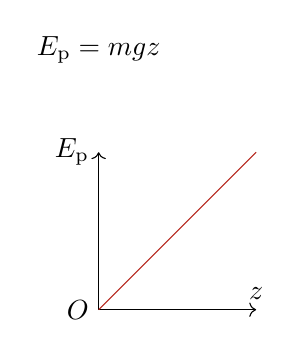
\begin{tikzpicture}
            \coordinate[label=left:$E_{\mathrm{p}}$] (E_p) at (0,2);
            \coordinate[label=above:$z$] (z) at (2,0);
            \coordinate[label=left:$O$] (O) at (0,0);
            \coordinate[label={above:$E_{\mathrm{p}} = mg z$}] (formula) at (0,3);
            \draw[->] (O) -- (z);
            \draw[->] (O) -- (E_p);
            \draw[domain=0:2,BrickRed] plot(\x,{\x});
        \end{tikzpicture}
    }
    \subfigure
    {
        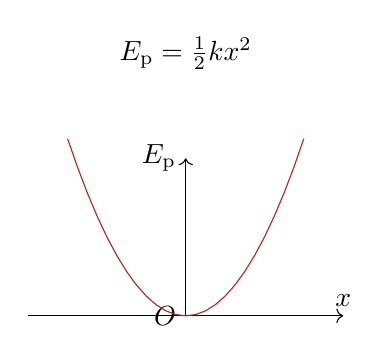
\begin{tikzpicture}
            \coordinate[label=left:$E_{\mathrm{p}}$] (E_p) at (0,2);
            \coordinate[label=above:$x$] (x) at (2,0);
            \coordinate[label=left:$O$] (O) at (0,0);
            \coordinate[label={above:$E_{\mathrm{p}} = \frac{1}{2}kx^2$}] (formula) at (0,3);
            \draw[->] (-2,0) -- (x);
            \draw[->] (O) -- (E_p);
            \draw[domain=-1.5:1.5,BrickRed] plot(\x,{\x*\x});
        \end{tikzpicture}
    }
    \subfigure
    {
        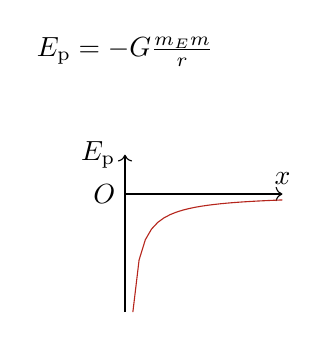
\begin{tikzpicture}
            \coordinate[label=left:$E_{\mathrm{p}}$] (E_p) at (0,0.5);
            \coordinate[label=above:$x$] (x) at (2,0);
            \coordinate[label=left:$O$] (O) at (0,0);
            \coordinate[label={above:$E_{\mathrm{p}} = -G \frac{m_{E}m}{r}$}] (formula) at (0,1.5);
            \draw[->] (O) -- (x);
            \draw[->] (0,-1.5) -- (E_p);
            \draw[domain=0.1:2,BrickRed] plot(\x,{-0.15/\x});
        \end{tikzpicture}
    }
    % \caption{}
\end{figure}

把势能和相对位置的关系绘成曲线,便得到势能曲线。
        
通过势能曲线,可以显示出系统总机械能,动能和势能间的关系
$E=E_k+E_p$,由 $E_{\mathrm{k}} \geq 0$ ,可以根据曲线的形状讨论物体的运动。

\subsubsection{由势能求表达式}

可以根据势能\(E_{\mathrm{p}}\left(x,y,z\right)\)的情况,判断物体在各个位置所受保守力的大小和方向:

$$
    \rmd W=F_x \rmd x=-\rmd E_p
$$

则

\begin{equation}
    F_x=-\frac{\rmd E_p}{\rmd x}
\end{equation}

如果势能是位置\(\left(x,y,z\right)\)的多元函数,则

\begin{equation}
    \overrightarrow{F}=F_x \overrightarrow{i}+F_y \overrightarrow{j}+F_z \overrightarrow{k}=
    -\left(\frac{\partial E_p}{\partial x} \overrightarrow{i}+\frac{\partial E_p}{\partial y} \overrightarrow{j}+\frac{\partial E_p}{\partial z} \overrightarrow{k}\right)
\end{equation}

\subsection{成对的力的功}

力总是成对的,无论是保守力还是非保守力。

设质量为$m_1$和$m_2$的两个物体分别受到 $F_1$ 和 $F_2$ 的力,
且 $\overrightarrow{F}_1=-\overrightarrow{F}_2$在$\rmd t$时间内位移为 $\rmd r_1$
和 $\rmd r_2$ ,质点 2 相对于质点 1 的相对位移 $\rmd \overrightarrow{r}^{\prime}$有
$\rmd \overrightarrow{r}_2=d \overrightarrow{r}_1+\rmd r^{\prime}$ 则元功为:

$$
    \begin{aligned}
    & \rmd W_1=\overrightarrow{F}_1 \cdot \rmd \overrightarrow{r}_1 \\
    & \rmd W_2=\overrightarrow{F}_2 \cdot \rmd \overrightarrow{r}_2
    \end{aligned}
$$

这一对力所作元功之和为:

$$
\begin{aligned}
    & \rmd W=\overrightarrow{F}_1 \cdot \rmd \overrightarrow{r}_1+\overrightarrow{F}_2 \cdot \rmd \overrightarrow{r}_2=\overrightarrow{F}_1 \cdot\rmd\overrightarrow{r}_1+\overrightarrow{F}_2 \cdot\left(d \overrightarrow{r}_1+d \overrightarrow{r}^{\prime}\right) \\
    & =\left(-\overrightarrow{F}_2+\overrightarrow{F}_2\right) \cdot\rmd\overrightarrow{r}_1+\overrightarrow{F}_2 \cdot\rmd\overrightarrow{r}^{\prime} \quad \\
    & =\overrightarrow{F}_2 \cdot\rmd\overrightarrow{r}^{\prime}
\end{aligned}
$$

\begin{enumerate}
    \item 成对力的功只与作用力和相对位移有关;
    \item 成对力的总功具有与参考系选择无关的不变性质。\\
        为方便起见,计算时常认为其中一个质点静止,并以该质点所在位置为原点,
        再计算另一质点受力所做的功,这就是一对力的功。
    \item 在无相对位移或相对位移与一对力垂直的情况下,一对力的功必为零。
\end{enumerate}

\section{功能原理、机械能守恒定律}

\subsection{质点系功能原理}

\textbf{系统的机械能}:动能与势能的综合称为机械能,即

\[
    E = E_{\mathrm{k}} + E_{\mathrm{p}}
\]

\textbf{内力的功可分为}:保守内力的功和非保守内力功

\[
    W^{\mathrm{in}} = \sum_{i} W_{i}^{\mathrm{in}} =
    W_{\mathrm{c}}^{\mathrm{in}} + W_{\mathrm{nc}}^{\mathrm{in}}
\]

由势能的定义,保守内力的功总等于系统势能的减少:

\[
    W_{\mathrm{c}}^{\mathrm{in}} = - \Delta E_{\mathrm{p}}
\]

\textbf{系统的功能原理}

(由质点系的动能定理)

\[
    W^{\mathrm{ex}} + W^{\mathrm{in}} = W^{\mathrm{ex}} + W_{\mathrm{c}}^{\mathrm{in}}
    + W_{\mathrm{nc}}^{\mathrm{in}} = W^{\mathrm{ex}} - \Delta E_{\mathrm{p}} +
    W_{\mathrm{nc}}^{\mathrm{in}} = \Delta E_{\mathrm{k}}
\]

于是,

\begin{align}
    \Delta E = \Delta E_{\mathrm{k}} + \Delta E_{\mathrm{p}} =
    W^{\mathrm{ex}} + W_{\mathrm{nc}}^{\mathrm{in}}
\end{align}

在选定的质点系内,在任一过程中,质点系总机械能的增量等于\textbf{所有外力}的功与\textbf{非保守内力}的功的代数和。

非保守内力的功将导致机械能与其他形式的能量转换。

\subsection{机械能守恒定律}

由功能原理:$\Delta E = \Delta E_{\mathrm{k}} + \Delta E_{\mathrm{p}} =
W^{\mathrm{ex}} + W_{\mathrm{nc}}^{\mathrm{in}}$。

如果$W^{\mathrm{ex}} + W_{\mathrm{nc}}^{\mathrm{in}} = 0$,则

\[
    \Delta E = \Delta E_{\mathrm{k}} + \Delta E_{\mathrm{p}} = 0
\]

即,如是系统内只有保守内力做功,其他内力和一切外力都不做功,或元功之和为零,
则系统内各物体的动能和势能可以相互转换,但总机械能保持不变。

\begin{enumerate}
    \item 质点系的机械能守恒的条件是:在一个过程中,既没有外力做功,也没有非保守内力(如摩擦力、爆炸力、流体的黏性阻力等耗散力)做功,或者外力和非保守内力做的总功为零。
    \item 在满足守恒条件时,质点系的总机械能可以在动能和系统势能之间转化,也可以在系统内各物体之问转移,但在转化和转移过程中保特总机械能不变。
\end{enumerate}

\subsection{能量守恒定律}

对于一个不受外界影响的封闭系统(有时也称为狐立系统),系统内各种不同形式的能量可以互相转化,也可以从系统的一部分转移到另一部分,
但不论系统内发生什么过程,能量既不会消失也不会产生,系统的总能量恒定不变。这就是能量守恒定律 (law of conservation of energy)。

\subsection{动量与能量的比较}

\begin{table}[htbp]
    \centering
    \begin{tabular}{|l|ll|}
        \hline
        \textbf{物理量} & \multicolumn{1}{l|}{\textbf{动量(momentum)}}                    & \textbf{能量(kinetic energy)}      \\ \hline
        表达式          & \multicolumn{1}{l|}{\(\overrightarrow{p} = m\overrightarrow{v}\)} & \(E_{\mathrm{k}} = \frac{1}{2}mv^2\) \\ \hline
        单位  & \multicolumn{1}{l|}{\(\mathrm{kg \cdot m / s}\)} & \(\mathrm{J}\)                  \\ \hline
        性质  & \multicolumn{1}{l|}{矢量}                      & 标量                          \\ \hline
        关系  & \multicolumn{2}{c|}{\(\dfrac{p^2}{2m} = E_{\mathrm{k}}\)}                       \\ \hline
        变化量 & \multicolumn{1}{l|}{\(\Delta p\)由力的冲量决定}         & \(\Delta E_{\mathrm{k}}\)由力的功决定 \\ \hline
    \end{tabular}
\end{table}

另外,\(\Delta p\)与惯性系的选择无关,\(\Delta E_{\mathrm{k}}\)随惯性系的不同而不同。

\section{碰撞、碰撞定律、质心运动定律}

\subsection{碰撞}

\textbf{定义}

两个或两个以上的物体相遇,相遇时物体之间的相互作用,仅持续极为短暂的时间。

\textbf{特点}

\begin{enumerate}
    \item 作用时间极短;
    \item 作用力变化极快;
    \item 作用力峰值极大;
    \item 过程中物体发生形变;
    \item 可认为碰撞过程中只受内力(\(\overrightarrow{F}^{\mathrm{ex}} \ll \overrightarrow{F}^{\mathrm{in}}\)),故遵守动量守恒定律(\(\sum_{i} \overrightarrow{p}_{i} = \overrightarrow{C}\))。
\end{enumerate}

\subsection{碰撞定律}

\begin{align}
    e = \frac{v_2 - v_1}{v_{10} - v_{20}}
\end{align}

即

$$
e = \frac{\text{分离速度}}{\text{接近速度}}
$$

(\(e\)称恢复系数,由材料性质决定。)

\subsection{碰撞的分类}

\subsubsection{完全弹性碰撞}

恢复系数\(e=1\),\(v_2-v_1=v_{10} - v_{20}\)。

碰撞后形变能完全恢复,没有机械能的损失,系统碰撞前后机械能守恒。

动量守恒,机械能守恒。

对于\textbf{完全弹性对心碰撞}:

$$
    \left\{\begin{array}{l}
    m_1 v_{10}+m_2 v_{20}=m_1 v_1+m_2 v_2 \\
    \dfrac{1}{2} m_1 v_{10}^2+\dfrac{1}{2} m_2 v_{20}^2=\dfrac{1}{2} m_1 v_1^3+\dfrac{1}{2} m_2 v_2^2
    \end{array}\right.
$$

联立方程解得

\begin{align}
    \left\{\begin{array}{l}
        v_1=\dfrac{m_1-m_2}{m_1+m_2} v_{10}+\dfrac{2 m_2}{m_1+m_2} v_{20} \\
        v_2=\dfrac{2 m_1}{m_1+m_2} v_{10}+\dfrac{m_2-m_1}{m_1+m_2} v_{20}
    \end{array}\right.
\end{align}

\subsubsection{完全非弹性碰撞}

恢复系数\(e=0\),\(v_2=v_1=v\)。

碰撞后二者没有分开,并以共同的速度一起运动。物体碰撞后已经完全不可能恢复形变。

动量守恒,机械能不守恒。

对于\textbf{完全非弹性对心碰撞}:

由

$$
    m_1 v_{10}+m_2 v_{20}=\left(m_1+m_2\right) v
$$

解得

\begin{equation}
    v=\frac{m_1 v_{10}+m_2 v_{20}}{m_1+m_2}
\end{equation}

损失能量

\begin{equation}
    \Delta E=\frac{1}{2} m_1 v_{10}^2+\frac{1}{2} m_2 v_{20}^2-\frac{1}{2}\left(m_1+m_2\right) v^2
\end{equation}

\subsubsection{非完全弹性碰撞}

恢复系数\(0<e<1\),\(v_2=v_1=e\left(v_{10} - v_{20}\right)\)。

碰撞后形变不能完全恢复,一部分机械能将被转变为其他形式的能量(如热能)。

动量守恒,机械能不守恒。

\subsubsection{斜碰撞}

碰撞前与碰撞后的速度不在一条直线上。

例如,一光滑球与另外静止的光滑球相碰。如果两者均为弹性球,且碰后两者的运动方向垂直,
则两小球质量必然相等

\subsection{质心}

\subsubsection{定义}

在研究质点系统问题中,与质点系统质量分布有关的一个代表点,它的位置在平均意义上代表
着质量分布中心。

\subsubsection{质心位置}

\begin{align}
    \overrightarrow{r}_{\mathrm{C}} = \frac{\sum_{i} m_ir_i}{M}
\end{align}

即

$$
    \left\{\begin{array}{l}
    x_C=\frac{\sum m_i x_i}{M} \\
    y_C=\frac{\sum m_i y_i}{M} \\
    z_C=\frac{\sum m_i z_i}{M}
    \end{array}\right.
$$

则质量连续分布的系统的质心位置

$$
    \overrightarrow{r}_C=\int \overrightarrow{r} \rmd m / M
$$

即

$$
    \left\{\begin{array}{l}
        x_c=\frac{\int x \mathrm{~d} m}{M} \\
        y_c=\frac{\int y \mathrm{~d} m}{M} \\
        z_c=\frac{\int z \mathrm{~d} m}{M}
    \end{array}\right.
$$

\textbf{注意}

\begin{enumerate}
    \item 质心不同于重心,物体体积不太大时,两者重和;物体远离地球时不受重力,"重心"失去意义,"质心"仍在。
    \item 当外力的作用线通过质心时,物体只作平动,没有转动,就好像物体的质量都集中在质心这一点上。
\end{enumerate}

\subsubsection{质心速度}

\begin{equation}
    \overrightarrow{v}_C=\frac{\rmd \overrightarrow{r}_C}{\rmd t}=\frac{\sum m_i \frac{\rmd \overrightarrow{r}_i}{\rmd t}}{M}=\frac{\sum m_i \overrightarrow{v}_i}{M}
\end{equation}

\subsubsection{质心加速度}

\begin{equation}
    \overrightarrow{v}_C=\frac{\rmd \overrightarrow{r}_C}{\rmd t}=\frac{\sum m_i \frac{\rmd \overrightarrow{r}_i}{\rmd t}}{M}=\frac{\sum m_i \overrightarrow{v}_i}{M}
\end{equation}

\subsection{质心运动定律}

质心的加速度与质点系所受外力的矢量和成正比,与质点系的总质量成反比,质心的加速度与内力无关。

\begin{equation}
    \overrightarrow{a}_C=\frac{\sum \overrightarrow{F}_i}{\sum m_i}=\frac{\sum \overrightarrow{F}_i}{M}
\end{equation}


\section{例题}

\subsection{Problem 1}

\begin{wrapfigure}{r}{4cm}
    \centering
    \includegraphics[scale=0.12]{"Chapter 03 images/pic7.png"}
    % \caption{}
    \label{pic7}
\end{wrapfigure}

在宇宙中有密度为\(\rho\)的尘埃,这些尘埃相对惯性参考系是静止的。有一质量为\(m_0\)的宇宙飞船以初速度\(v_0\)
穿过宇宙尘埃,由于尘埃粘贴到飞船上,致使飞船的速度发生改变。求飞船的速度与其在尘埃中飞行时间的关系。
(设想飞船的外形是截面积为\(S\)的圆柱体)
\vspace{1em}

\textbf{Solution}
\vspace{1em}

尘埃与飞船作完全非弹性碰撞,把它们作为一个系统,则动量守恒:

$$
    m_0 v_0+\left(m-m_0\right) \times 0=m v
$$

解得

\[
    m = \frac{m_0v_0}{v}
\]

所有与飞船迎面相撞的尘埃都会粘贴到飞船上。考查\(\rmd t\)时间内与飞船迎面相撞的尘埃:

\[
    \rmd m = \rho Sv\rmd t
\]

又因为

\[
    m = \frac{m_0v_0}{v}
\]

所以

\[
    \rmd m = -\frac{m_0v_0}{v^2} \rmd v = \rho Sv\rmd t
\]

由

$$
    -\int_{v_0}^v \frac{d v}{v^3}=\frac{\rho S}{m_0 v_0} \int_0^t d t
$$

得

$$
    v=v_0\sqrt{\frac{m_0}{2 \rho S v_0 t+m_0}}
$$

\subsection{Problem 2}

\begin{wrapfigure}{r}{4cm}
    \centering
    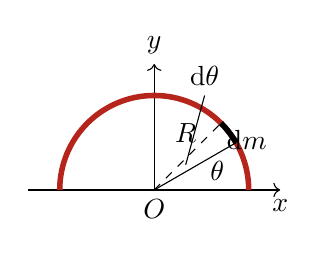
\begin{tikzpicture}[scale=0.8]
        \coordinate[label=below:$x$] (x) at (2,0);
        \coordinate[label=above:$y$] (y) at (0,2);
        \coordinate[label=below:$O$] (O) at (0,0);
        \draw[->] (O) -- (y);
        \draw[->] (-2,0) -- (x);
        \draw[BrickRed, line width=2pt] (1.5,0) arc (0:180:1.5);
        \draw[Black, line width=2pt] (0.75*1.732,0.75) arc (30:45:1.5);
        \draw[dashed] (O) -- (0.75*1.414,0.75*1.414);
        \draw (O) -- (0.75*1.732,0.75);
        \coordinate[label=above:$\theta$] (theta) at (1,0);
        \coordinate[label=above:$R$] (R) at (0.5,0.6);
        \coordinate[label=above:$\rmd \theta$] (dtheta) at (0.8,1.5);
        \draw (0.5,0.4) -- (dtheta);
        \coordinate[label=right:$\rmd m$] (dm) at (1,0.8);
    \end{tikzpicture}
\end{wrapfigure}

已知一圆环半径为\(R\),质量为\(M\),求它的质心位置。
\vspace{1em}

\textbf{Solution}
\vspace{1em}

建坐标系如图,取一小段长度\(\rmd l\)则其质量为\(\rmd m = \lambda \rmd l\)。

又\(\rmd l = R \rmd \theta\),故\(\rmd m = \frac{M}{\uppi R} R \rmd \theta\)

而\(x = R\cos \theta\),\(y = R\sin \theta\)

故

$$
    y_c=\frac{\int y \mathrm{~d} m}{M}=\frac{\int_0^\pi R \sin \theta \frac{M}{\pi R} R \mathrm{~d} \theta}{M}=\frac{2 R}{\pi}
$$

由对称性可知,

$$
    x_c = 0
$$

%----------------------------------------------------------------------------------------
%	PRESENTING INFORMATION/RESULTS EXAMPLES CHAPTER
%----------------------------------------------------------------------------------------

% \chapterimage{orange3.jpg} % Chapter heading image
% \chapterspaceabove{6.25cm} % Whitespace from the top of the page to the chapter title on chapter pages
% \chapterspacebelow{7.5cm} % Amount of vertical whitespace from the top margin to the start of the text on chapter pages

%----------------------------------------------------------------------------------------

\end{document}
